\subsection{Fonctionnalité 1}
La première fonctionnalité du système devra permettre les opérations conventionnelles de gestion individuelle comme la création d'un bénévole dans le système, la modification des caractéristiques le concernant et la suppression d'un bénévole. La suppression d'un bénévole devra être logique et non physique de façon à ne pas effacer l'historique des actions effectuées par ce bénévole. \\
Un bénévole sera identifié par son adresse électronique.\\ 
Un cas spécial sera prévu pour un bénévole spécial qui ne sera rattaché à aucune information personnelle mais dont les actions seront tracées.\\
Les informations associées à un bénévole sont :
\begin{itemize}
\item son identifiant (adresse électronique),
\item son mot de passe,
\item son nom,
\item son prénom,
\item son adresse postale,
\item son type (administrateur global, administrateur local ou bénévole),
\item son téléphone fixe et/ou mobile,
\item son ou ses domaines d'activités potentielles (si le bénévole en a),
\item sa ou ses responsabilités d'activité (si responsable).
\\
\end{itemize}

Les figures \ref{utilisateurNonConnecte} et \ref{utilisateurConnecte} présentent les diagrammes de cas d'utilisation propres aux actions possibles pour un utilisateur connecté et un utilisateur non connecté.\\
Les figures \ref{fonctionnalite1creationDUnUtilisateurs}, \ref{fonctionnalite1modificationDUnProfil}  et \ref{fonctionnalite1modificationDUnProfilAdmin} présentent respectivement la maquette de l'interface de création de profil et celles de la modification de profil (par un l'utilisateur puis par l'administrateur). \\
\begin{figure}[H]
	\centering
	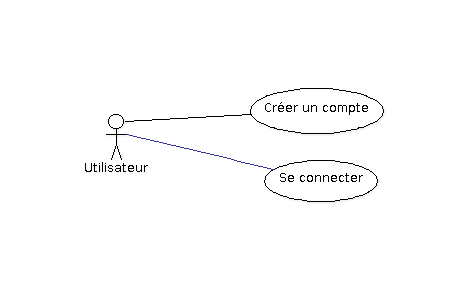
\includegraphics[scale=0.4]{images/casDUtilisation/fonctionnalite1UtilisateurNonConnecte.png}
	 \caption{Cas d'utilisation  d'un utilisateur non connecté}
	 \label{utilisateurNonConnecte}
\end{figure}

\begin{figure}[H]
	\centering
	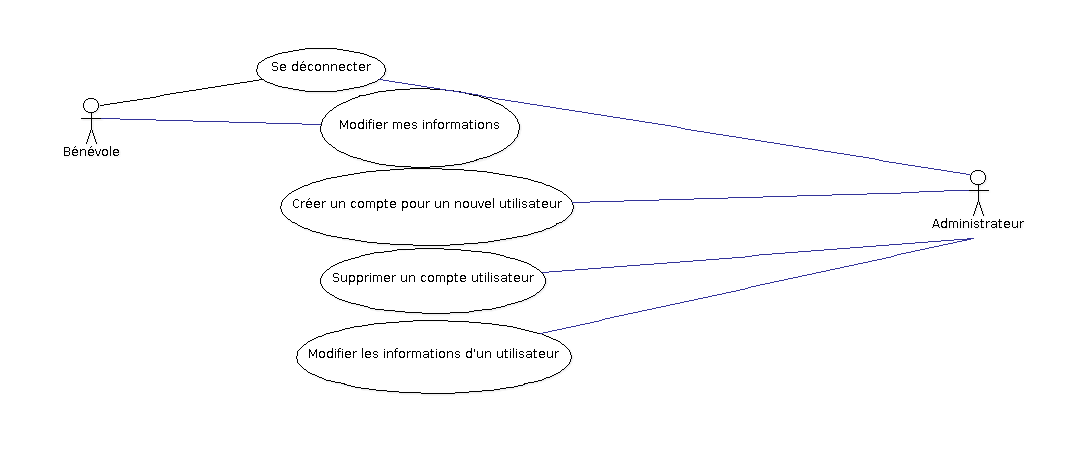
\includegraphics[scale=0.4]{images/casDUtilisation/fonctionnalite1UtilisateurConnecte.png}
	 \caption{Cas d'utilisation  d'un utilisateur connecté}
	 \label{utilisateurConnecte}

\end{figure}


% Figure : version 1.00, date 24/02/16, auteur Michel Cressant
\begin{figure}[H]
	\centering
	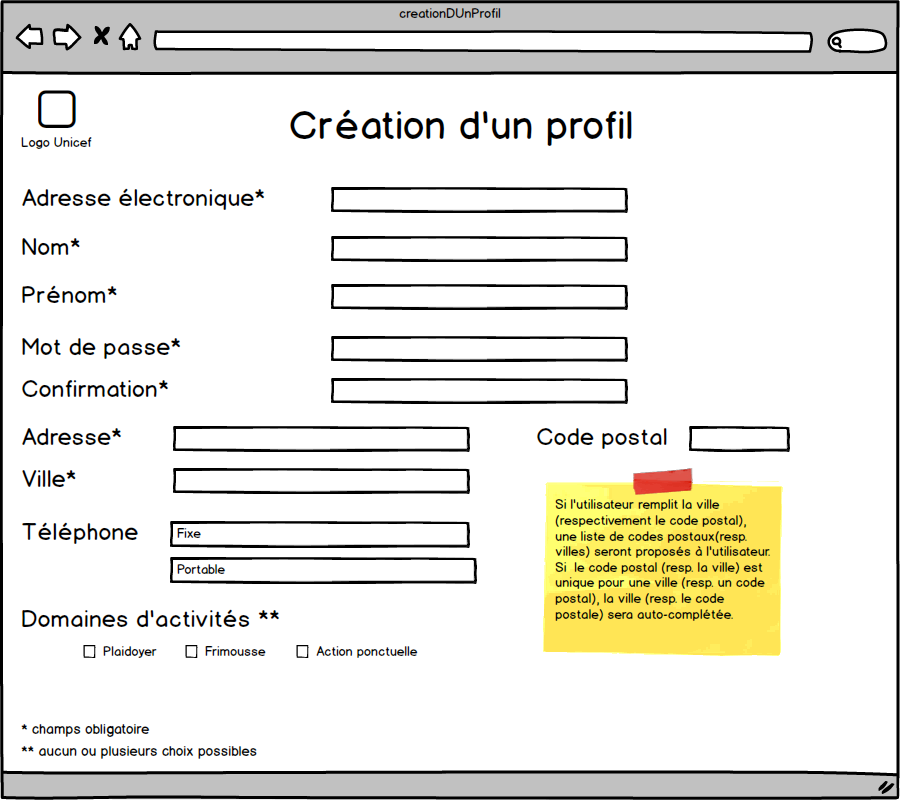
\includegraphics[scale=0.4]{images/maquettes/fonctionnalite1CreationDUnProfil.png}
	 \caption{Maquette~: Creation d'un utilisateur}
 \label{fonctionnalite1creationDUnUtilisateurs}
\end{figure}

% Figure : version 1.00, date 24/02/16, auteur Michel Cressant
\begin{figure}[H]
	\centering
	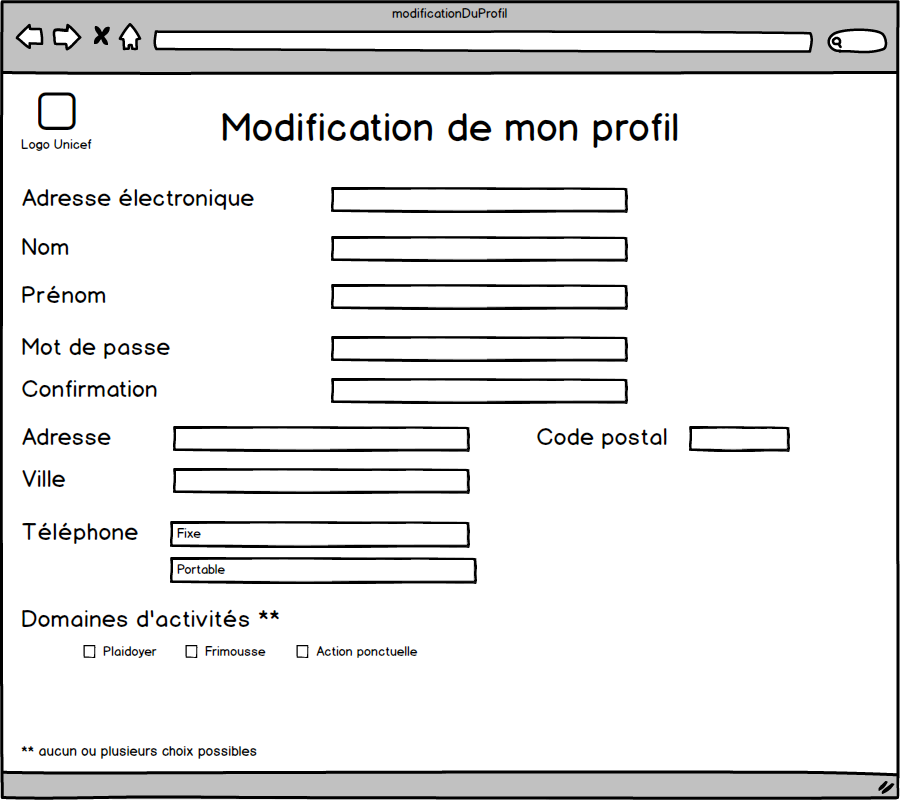
\includegraphics[scale=0.4]{images/maquettes/fonctionnalite1ModificationDUnProfil.png}
	 \caption{Maquette~: Modification des informations d'un utilisateur par l'utilisateur}
	 \label{fonctionnalite1modificationDUnProfil}
\end{figure}


% Figure : version 1.00, date 24/02/16, auteur Michel Cressant
\begin{figure}[H]
	\centering
	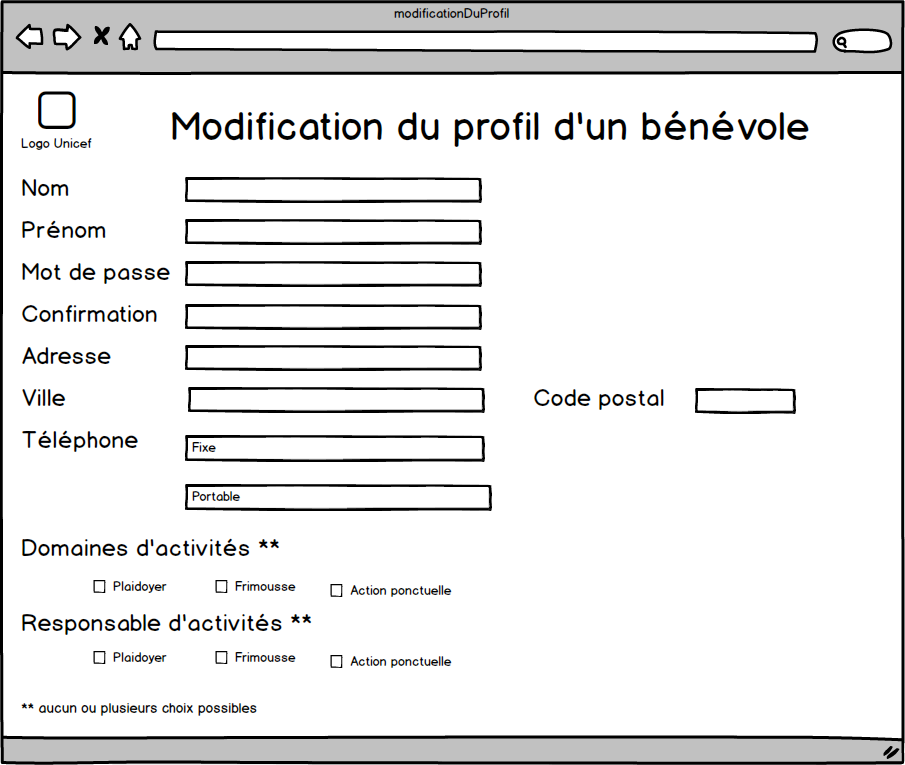
\includegraphics[scale=0.4]{images/maquettes/fonctionnalite1ModificationDUnProfilAdmin.png}
	 \caption{Maquette~: Modification des informations d'un utilisateur par l'administrateur}
	 \label{fonctionnalite1modificationDUnProfilAdmin}
\end{figure}

Un administrateur global est un utilisateur qui a tous les droits. \\ Un administrateur local est un responsable d'activité, il a des droits de lecture et de modification sur son activité. \\ Un bénévole a des droits de lecture et de modification sur ses informations personnelles et seulement des droits de lecture sur les informations concernant ses domaines d'activité. Il pourra également s'attribuer une activité, entrer et modifier des informations sur cette activité.\\
Il pourra exister plusieurs administrateurs globaux, plusieurs administrateurs locaux et plusieurs bénévoles. Un administrateur local peut être responsable de plusieurs activités.



Les activités potentielles pourront ainsi avoir plusieurs responsables et seront composées des actions ponctuelles, des plaidoyers et des actions frimousses. \\

Un ou plusieurs utilisateurs peuvent être responsable d'un, plusieurs ou aucun projets (école, lycéen ou étudiant).\\

La création et la modification d'une caractéristique concernant un bénévole devront faire l'objet d'un envoi de mail au bénévole l'informant de la création ou modification voulue et donnant l'ensemble des informations le concernant. Un an après une modification sur une caractéristique sur un utilisateur, l'ancienne caractéristique sera supprimée. \\


Une contrainte d'intégrité du système est que toute action effectuée doit avoir été réalisée par un bénévole existant. \\
Si le nom de l'intervenant ayant effectué une action n'est pas connu, l'action sera attribuée a un bénévole spécial. Une fonction d'interrogation permettant de donner la liste des interventions effectuées par ce bénévole fictif sera implémentée afin d'engager les actions nécessaires pour trouver le nom du bénévole ayant effectué cette action. \\


La procédure de connexion au système sera basée sur le couple login (adresse e-mail) / mot de passe.
